%!TEX TS-program = xelatex

% HSE Beamer Theme
% by Danil Fedorovykh
% http://hse.ru/staff/df
%
% Version 2.0 (English)
% January 2022

%%% Set up the free HSE Sans font
%%% https://www.hse.ru/info/brandbook/#font

\documentclass[aspectratio=169]{beamer}

\newbool{russian}
\booltrue{russian} % Uncomment if in Russian
\usepackage{HSE-theme/beamerthemeHSE} % Load HSE theme
\usepackage[no-math]{fontspec}      % fonts loading
\usepackage{caption}
\usepackage{subfigure}
\usepackage{subcaption}
\usepackage{hyperref}
\captionsetup[figure]{labelformat=empty}
\captionsetup[subfigure]{labelformat=empty}
\setsansfont{HSE Sans}
\graphicspath{{images/}}

%%% Информация об авторе и выступлении
\title[Title]{Алгоритмы и структуры данных} 
\subtitle{Лекция 0. Алгоритмы и программы}
\author[Author's name]{Илья Сергеевич Бычков\\ \smallskip \scriptsize \url{ibychkov@hse.ru}}
\institute{НИУ ВШЭ - Нижний Новгород}
\date{\today}


\begin{document}

\frame[plain]{\titlepage}

\begin{frame}
\frametitle{О курсе}
\framesubtitle{Оценивание}
Продолжительность курса: октябрь - июнь / 2-4 модули /9 месяцев\newline
Состав курса: \~ 30 лекций + 30 практик\newline\newline
Из чего складывается накопленная оценка:
\begin{itemize}
  \item{Контесты - \textcolor{red}{вес 0.3}}
  \item{Контрольные - \textcolor{red}{вес 0.6}}
  \item{Активность/доп задания - \textcolor{red}{вес 0.1}}
\end{itemize}
Оценка за модули 2-3 = Накопленная оценка * 0.6 + Экзамен * 0.4\newline
Оценка за модуль 4 = Накопленная оценка * 0.6 + Экзамен * 0.4\newline\newline
Финальная оценка = Оценка за модули 2-3 * 0.6 + Оценка за модуль 4 * 0.4
\end{frame}

\begin{frame}
\frametitle{О курсе}
\framesubtitle{Команда курса}
Лекции\newline \textcolor{blue}{Илья Сергеевич Бычков} - HSE PhD, Senior Algorithm Developer (Huawei), старший научный сотрудник ЛАТАС\newline\newline
Семинары:
\begin{itemize}
  \item{\textcolor{blue}{Максим Отчество Захаров} - Разработчик и тд}
  \item{\textcolor{blue}{Михаил Отчество Железин} - Разработчик и тд}
  \item{\textcolor{blue}{Андрей Отчество Сапожников} - Разработчик и тд}
  \item{\textcolor{blue}{Никита Отчество Наумов} - Разработчик и тд}
  \item{\textcolor{blue}{Вакансия Отчество Вакансия} - Разработчик и тд}
\end{itemize}
\end{frame}

\begin{frame}
\frametitle{О курсе}
\framesubtitle{Литература}

\begin{figure}
    \captionsetup[subfigure]{labelformat=empty}
    \centering
    \subfigure[\textbf{\newline Introduction to \newline Algorithms, 4th Edition}\newline Thomas H Cormen \newline Charles E Leiserson \newline Ronald L Rivest \newline Clifford Stein]{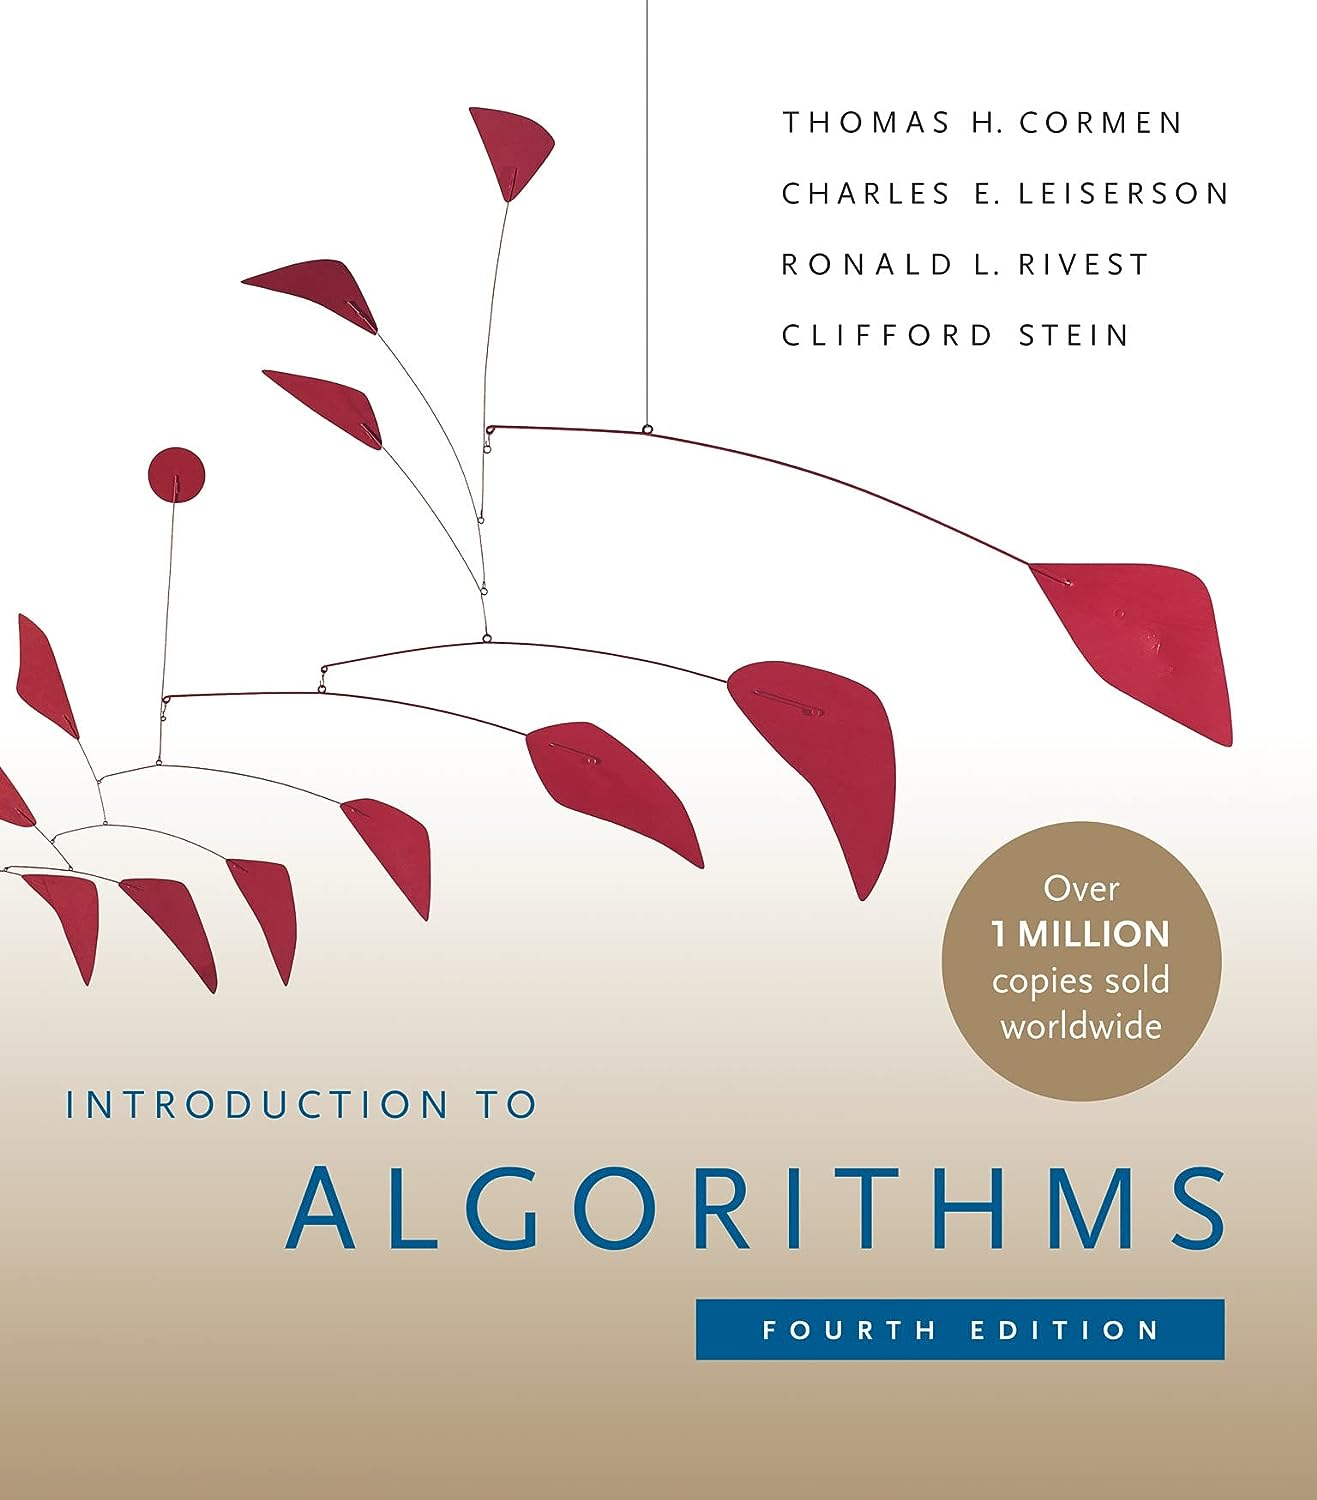
\includegraphics[width=0.24\textwidth]{cormen_4_cover}} 
    \subfigure[\textbf{\newline Algorithms}\newline Sanjoy Dasgupta \newline Christos Papadimitriou \newline Umesh Vazirani ]{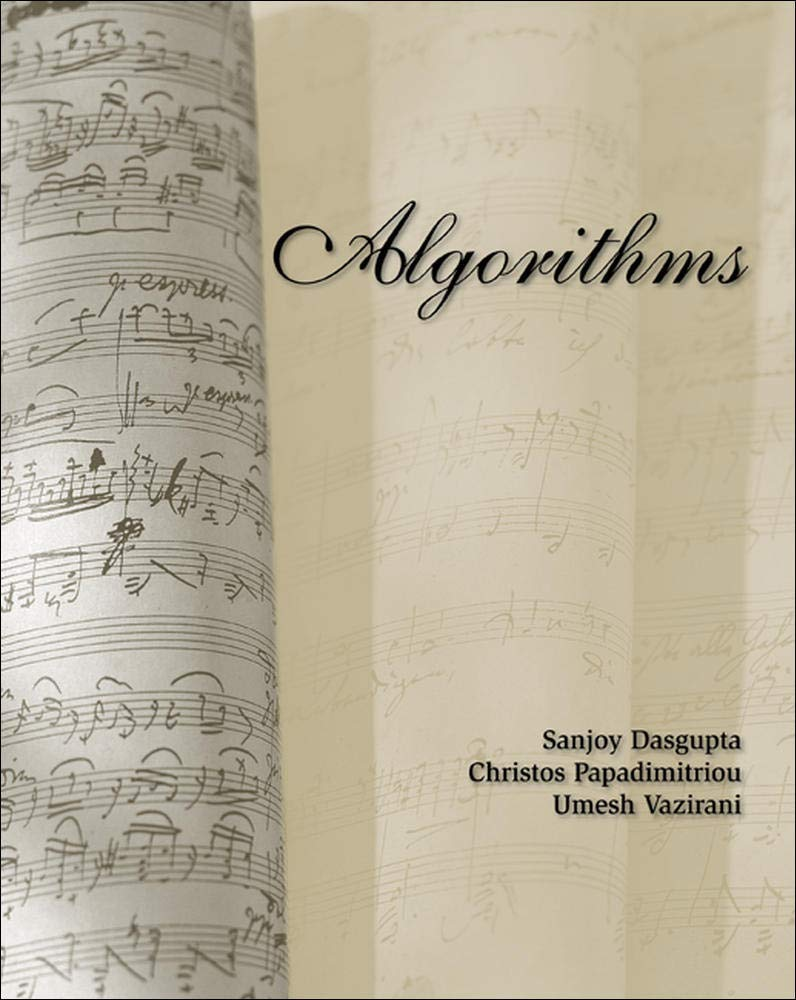
\includegraphics[width=0.24\textwidth]{dasgupta_cover}} 
    \subfigure[\textbf{\newline Algorithms, 4th Edition}\newline Robert Sedgewick \newline Kevin Wayne\newline \newline \url{algs4.cs.princeton.edu}]{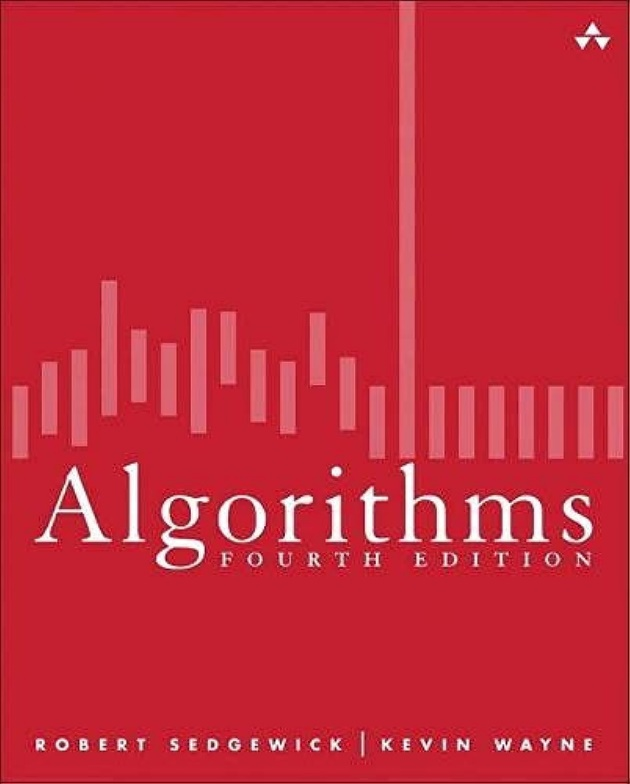
\includegraphics[width=0.24\textwidth]{sedgewick_cover}} 
    \subfigure[\textbf{Introduction to Algorithms, 4th Edition}\newline Thomas H Cormen, Charles E Leiserson, Ronald L Rivest, Clifford Stein]{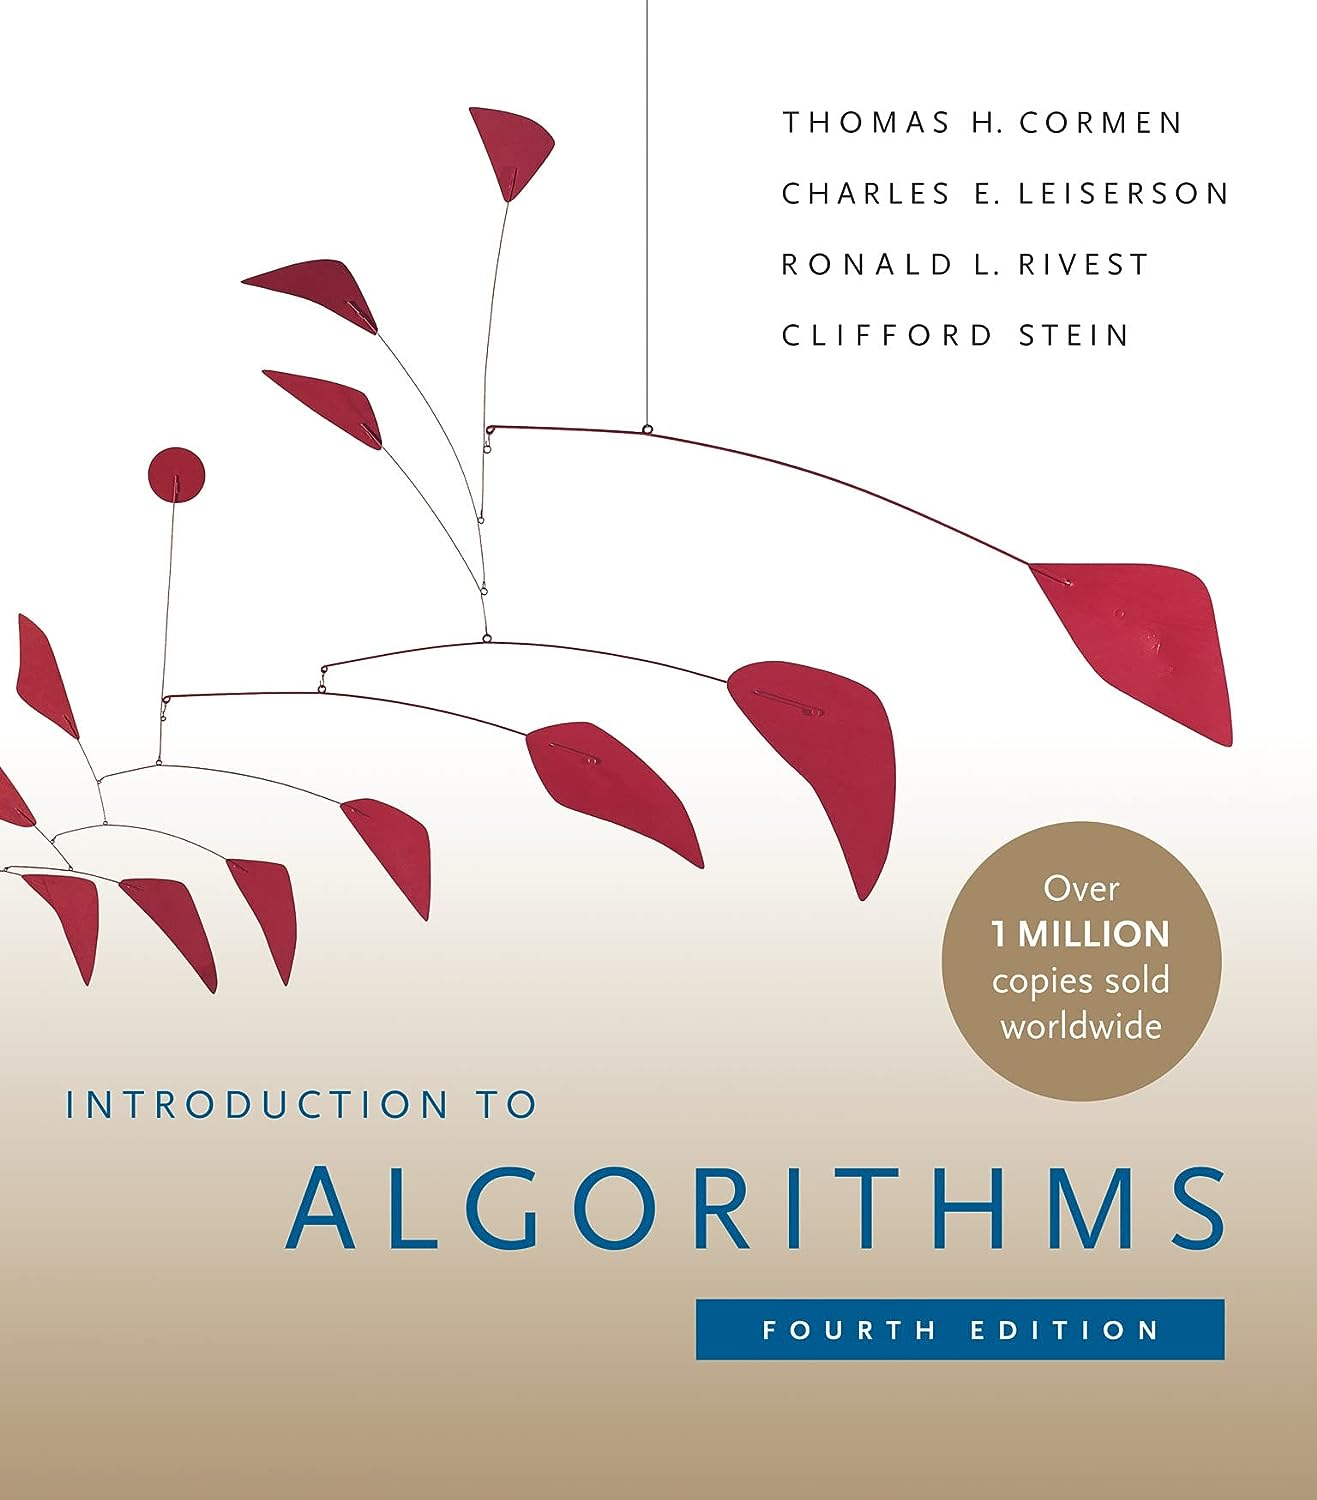
\includegraphics[width=0.24\textwidth]{cormen_4_cover}} 
    \label{fig:foobar}
\end{figure}
\end{frame}
\end{document}